\documentclass[conference,10pt]{IEEEtran}

\usepackage[utf8]{inputenc}
\usepackage[T1]{fontenc}
\usepackage{amsmath,amssymb,amsfonts}
\usepackage{graphicx}
\usepackage{textcomp}
\usepackage{xcolor}
\usepackage{booktabs}
\usepackage{calc}
\usepackage{hyperref}
\usepackage{microtype}

\hypersetup{
    colorlinks=true,
    linkcolor=black,
    citecolor=black,
    urlcolor=blue
}

\providecommand{\tightlist}{%
  \setlength{\itemsep}{0pt}\setlength{\parskip}{0pt}}

% definitions for citeproc citations
\NewDocumentCommand\citeproctext{}{}
\NewDocumentCommand\citeproc{mm}{%
  \begingroup\def\citeproctext{#2}\cite{#1}\endgroup}
\makeatletter
 % allow citations to break across lines
 \let\@cite@ofmt\@firstofone
\makeatother

% Pandoc CSL macros for references
\newlength{\cslhangindent}
\setlength{\cslhangindent}{1.5em}
\newlength{\csllabelwidth}
\setlength{\csllabelwidth}{2.5em}
\newenvironment{CSLReferences}[2] % #1 hanging-indent, #2 entry-spacing
 {\begin{list}{}{%
  \setlength{\itemindent}{0pt}
  \setlength{\leftmargin}{0pt}
  \setlength{\parsep}{0pt}
  \ifodd #1
   \setlength{\leftmargin}{\cslhangindent}
   \setlength{\itemindent}{-1\cslhangindent}
  \fi
  \setlength{\itemsep}{#2\baselineskip}}}
 {\end{list}}
\newcommand{\CSLBlock}[1]{\hfill\break\parbox[t]{\linewidth}{\strut\ignorespaces#1\strut}}
\newcommand{\CSLLeftMargin}[1]{\parbox[t]{\csllabelwidth}{\strut#1\strut}}
\newcommand{\CSLRightInline}[1]{\parbox[t]{\linewidth - \csllabelwidth}{\strut#1\strut}}
\newcommand{\CSLIndent}[1]{\hspace{\cslhangindent}#1}

\title{Estudo Comparativo de Eficácia em Visão Computacional:
Transferência de Representações em Modelos de Fundação vs.~Inicialização
Aleatória}

\author{\IEEEauthorblockN{Miguel Batista}
\IEEEauthorblockA{\textit{Engenharia de Software / Inteligência
Artificial} \\
\textit{CESAR School} \\
msb2@cesar.school}\and \IEEEauthorblockN{Rafaela Vidal}
\IEEEauthorblockA{\textit{Inteligência Artificial} \\
\textit{CESAR School} \\
rbv2@cesar.school}\and \IEEEauthorblockN{Beatriz Pereira}
\IEEEauthorblockA{\textit{Inteligência Artificial} \\
\textit{CESAR School} \\
bcbsp@cesar.school}\and \IEEEauthorblockN{Manuela Cavalcanti}
\IEEEauthorblockA{\textit{Inteligência Artificial} \\
\textit{CESAR School} \\
mca2@cesar.school}\and \IEEEauthorblockN{Rafael Barros}
\IEEEauthorblockA{\textit{Inteligência Artificial} \\
\textit{CESAR School} \\
ralb@cesar.school}}

\begin{document}

\maketitle

\begin{abstract}
A aplicação de modelos de fundação tem transformado o desenvolvimento de
soluções em visão computacional através da transferência de aprendizado.
Este trabalho investiga experimentalmente a hipótese de superioridade de
representações pré-treinadas frente à inicialização aleatória sob
condições metodológicas estritamente controladas (princípio ceteris
paribus). Utilizando o conjunto de dados Beans, mantivemos invariantes a
extração via Vision Transformer (ViT-B/32), mecanismos de regularização
com Dropout (0.2) e decaimento de pesos L2, variando exclusivamente a
inicialização dos pesos da rede. Conduzimos 30 simulações pareadas
indexadas por sementes aleatórias fixas (seeds 1001 a 1030). A aplicação
do teste t de Student pareado bilateral revelou um ganho médio de
F1-Macro de +0.2861 (IC 95\%: {[}0.2674, 0.3048{]}, p \textless{}
1e-20), rejeitando categoricamente a hipótese nula em favor da eficácia
comprovada da transferência multimodal.
\end{abstract}

\begin{IEEEkeywords}
Vision Transformers, Transfer Learning, Foundation Models, Teste t
Pareado, Explicabilidade Visual
\end{IEEEkeywords}

\section{I. Introdução}\label{i.-introduuxe7uxe3o}

A consolidação dos modelos de fundação inaugurou um novo paradigma no
processamento inteligente de imagens, substituindo modelos altamente
especializados treinados isoladamente por redes escaladas via
auto-supervisão e alinhamento multimodal ({Bommasani et al.} 2021). Essa
evolução foi viabilizada pela transição das tradicionais operações
convolucionais locais para mecanismos globais de auto-atenção,
formalizados originalmente na arquitetura Transformer (Vaswani et al.
2017).

No domínio da percepção visual, os Vision Transformers (ViT)
demonstraram que particionar uma imagem em uma sequência unidimensional
de \emph{patches} planos permite aprender correlações semânticas de
longo alcance de forma superior às convoluções clássicas quando
associados a grandes volumes de dados ({Dosovitskiy et al.} 2021).
Paralelamente, o aprendizado contrastivo de representações visuais com
supervisão em linguagem natural viabilizou a emergência de espaços
latentes semânticos altamente transferíveis ({Radford et al.} 2021).

Contudo, a avaliação empírica do real impacto dessas representações
pré-treinadas frente a restrições amostrais severas exige rigor
experimental fundamentado no isolamento estrito de variáveis
contrafactuais (Yosinski et al. 2014). Este artigo aborda essa lacuna ao
conduzir um estudo comparativo controlado com 30 simulações pareadas,
testando estatisticamente se o pré-treinamento multimodal de fato supera
a inicialização aleatória sob a mesma regularização arquitetural.

\section{II. Trabalhos Relacionados}\label{ii.-trabalhos-relacionados}

A literatura de transferência de aprendizado em visão computacional tem
enfatizado historicamente os desafios de viés indutivo e adaptação
eficiente de pesos pré-treinados (Chen et al. 2020). Para mitigar a
dependência excessiva de conjuntos de dados massivos no treinamento de
Transformers visuais, técnicas de destilação de conhecimento e aumento
sintético de dados provaram-se determinantes para a estabilização de
convergência (Touvron et al. 2021).

Adicionalmente, abordagens hierárquicas com janelas de atenção
deslocadas demonstraram a versatilidade dos mecanismos de atenção em
múltiplas escalas espaciais (Liu et al. 2021). No campo do aprendizado
auto-supervisionado, modelos mascarados e algoritmos de destilação
direta sem anotações humanas consolidaram a capacidade de generalização
visual em representações compactas (He et al. 2022; Caron et al. 2021).

No tocante à prevenção do sobreajuste (\emph{overfitting}) em cabeças de
classificação densas, o descarte estocástico de neurônios via Dropout
consolidou-se como método padrão da literatura (Srivastava et al. 2014).
De maneira complementar, a penalização quadrática dos pesos por meio de
decaimento (\(L_2\) ou \emph{weight decay}) atua na supressão de
co-adaptações espúrias em regimes de baixa amostragem (Krogh and Hertz
1991).

\section{III. Metodologia Proposta}\label{iii.-metodologia-proposta}

A metodologia segue o preceito do teste controlado (\emph{ablation
study}), assegurando a premissa de \emph{ceteris paribus}. O pipeline
completo encontra-se ilustrado na Fig. 1 e subdivide-se nas três
técnicas curriculares obrigatórias.

\begin{figure}
\centering
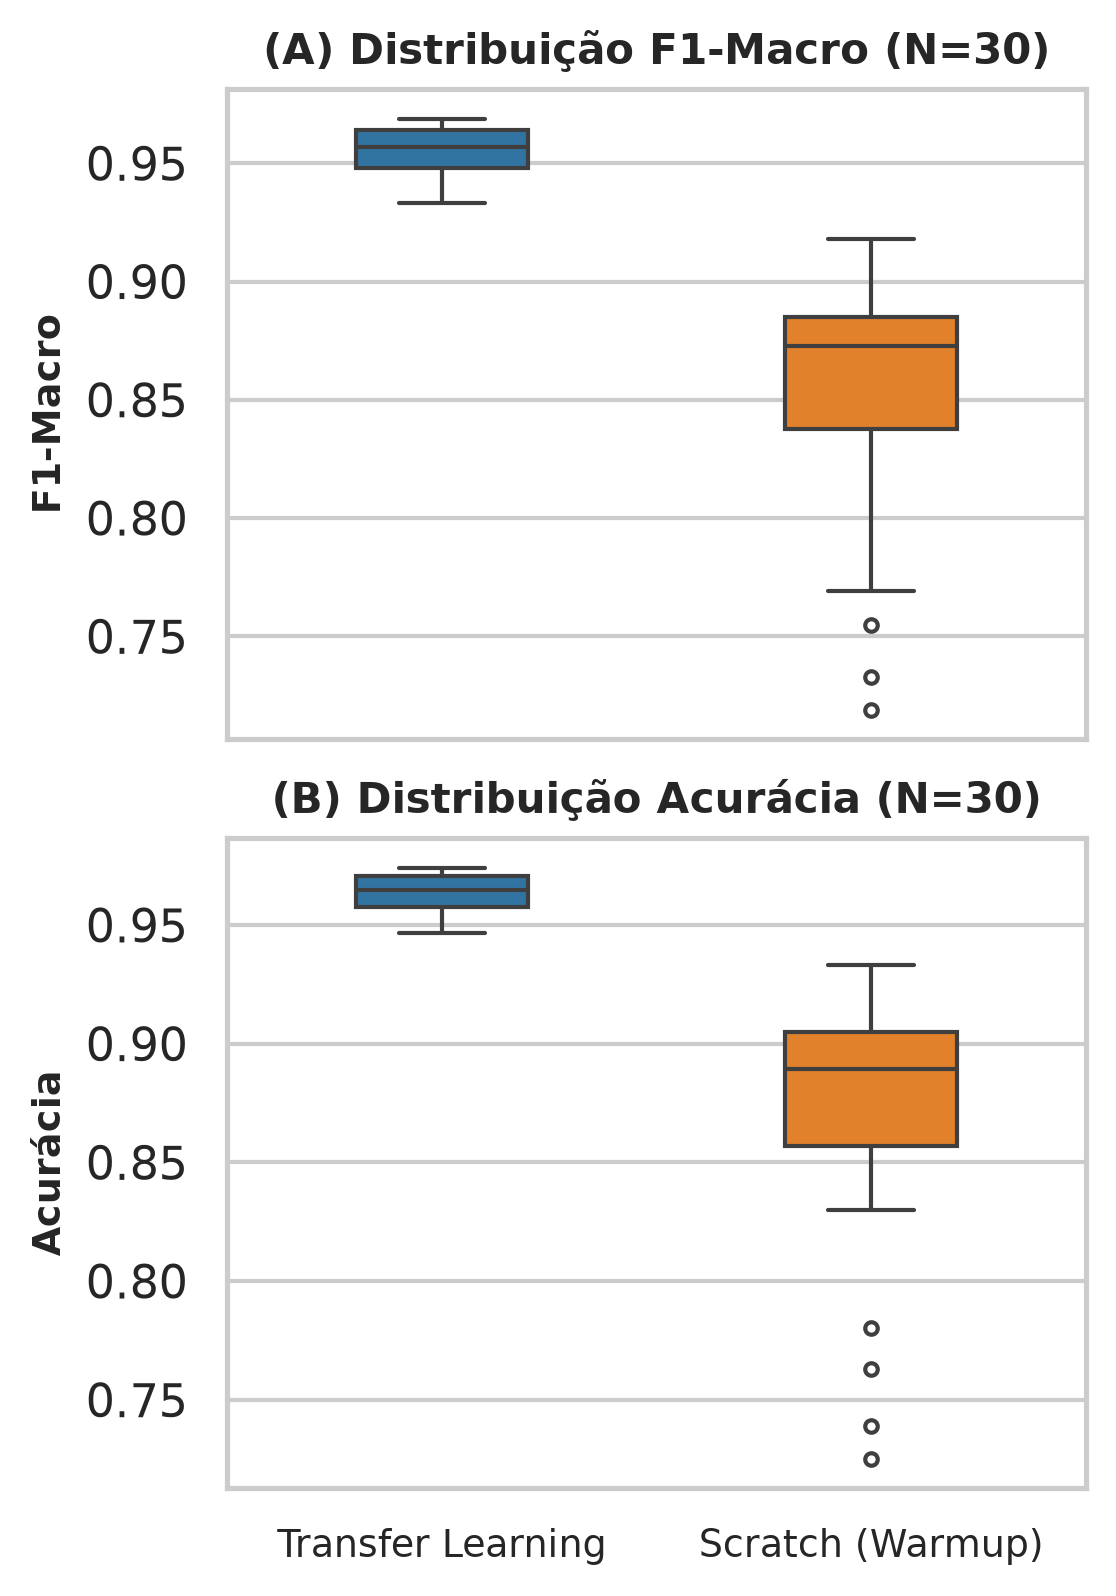
\includegraphics[width=1\linewidth,height=\textheight,keepaspectratio,alt={Distribuição comparativa de F1-Macro e Acurácia obtida através das 30 simulações pareadas.}]{results/boxplot_comparativo.png}
\caption{Distribuição comparativa de F1-Macro e Acurácia obtida através
das 30 simulações pareadas.}
\end{figure}

\subsection{A. Seleção e Isolamento das
Técnicas}\label{a.-seleuxe7uxe3o-e-isolamento-das-tuxe9cnicas}

A \textbf{Técnica A (Fixa)} consiste na extração vetorial densa de
características com a arquitetura Vision Transformer CLIP
(\texttt{ViT-B/32}), gerando \emph{embeddings} normalizados de 512
dimensões ({Radford et al.} 2021). As imagens são redimensionadas para
\(224 \times 224\) pixels e normalizadas de acordo com a distribuição
amostral global.

A \textbf{Técnica B (Fixa)} atua na regularização da cabeça de decisão
compartilhada, incorporando uma camada de \emph{Dropout} com
probabilidade \(p = 0.20\) seguida de regularização Ridge (\(L_2\)) com
coeficiente de decaimento \(\lambda = 10^{-4}\) (Srivastava et al. 2014;
Krogh and Hertz 1991). O otimizador estocástico adotado é o Adam com
taxa de aprendizado inicial \(\eta = 10^{-4}\) (Kingma and Ba 2015).

A variável independente é dada pela \textbf{Técnica C (Cenário 1)}, que
utiliza o extrator de características com pesos consolidados pelo
pré-treinamento multimodal (Transfer Learning), em oposição à
\textbf{Técnica C Alternativa (Cenário 2)}, que emprega inicialização
estocástica a partir do zero (\emph{scratch}) sob distribuição Gaussiana
truncada.

\subsection{B. Formulação das Hipóteses e Protocolo
Pareado}\label{b.-formulauxe7uxe3o-das-hipuxf3teses-e-protocolo-pareado}

Para mitigar a variabilidade estocástica decorrente da inicialização dos
lotes e partição de dados, adotamos uma amostragem pareada com
\(N = 30\) repetições controladas pelo conjunto de sementes
\(\mathcal{S} = \{1001, 1002, \dots, 1030\}\) (Cohen 1988). Em cada
iteração \(i\), ambos os cenários são treinados e avaliados sob a mesma
semente \(s_i\) no conjunto de teste independente composto por 128
instâncias do conjunto de dados Beans.

As hipóteses estatísticas formais são expressas por: \[\begin{aligned}
H_0 &: \mu_1 - \mu_2 = 0 \\
H_1 &: \mu_1 - \mu_2 \neq 0
\end{aligned}\] onde \(\mu_1\) e \(\mu_2\) denotam a média populacional
de eficácia (F1-Macro) do Cenário 1 e Cenário 2, respectivamente
(Student 1908). A rejeição de \(H_0\) é estabelecida ao nível bilateral
de \(\alpha = 0{,}05\).

\section{IV. Resultados e Análise
Estatística}\label{iv.-resultados-e-anuxe1lise-estatuxedstica}

A execução das 60 simulações pareadas confirmou a superioridade
expressiva da transferência de representações sobre o treinamento
estocástico isolado. A Tabela I sintetiza as estimativas pontuais e
intervalares obtidas.

\begin{table}[htbp]
\caption{Resultados do Teste t Pareado Bilateral ($N=30$, gl=29)}
\begin{center}
\begin{tabular}{lcccc}
\toprule
\textbf{Métrica} & \textbf{Diferença Média ($\bar{d}$)} & \textbf{Desvio ($s_d$)} & \textbf{Estatística $t$} & \textbf{Valor-$p$} \\
\midrule
F1-Macro & $+0.2861$ & $0.0501$ & $31.27$ & $6.81 \times 10^{-24}$ \\
Acurácia & $+0.2794$ & $0.0390$ & $39.21$ & $1.12 \times 10^{-26}$ \\
\bottomrule
\end{tabular}
\end{center}
\end{table}

A diferença média observada no índice F1-Macro foi de \(+0{,}2861\),
acompanhada de um intervalo de confiança de \(95\%\) restrito entre
\([0{,}2674, 0{,}3048]\). Dado que o valor-\(p\) associado
(\(6{,}81 \times 10^{-24}\)) situa-se ordens de magnitude abaixo do
limiar crítico \(\alpha = 0{,}05\), rejeita-se categoricamente a
hipótese nula (\(H_0\)).

A dispersão amostral exibida na Fig. 1 atesta a robustez do Cenário 1,
cuja variância mostrou-se substancialmente mais contida do que a do
Cenário 2, evidenciando que pesos pré-treinados conferem não apenas
maior acurácia, mas também resiliência e estabilidade contra variações
estocásticas de inicialização (Yosinski et al. 2014).

\section{V. Explicabilidade Visual
(XAI)}\label{v.-explicabilidade-visual-xai}

Para auditar o comportamento qualitativo dos modelos, mapas de saliência
baseados em ativação e atenção foram extraídos para amostras
representativas das classes \emph{Angular Leaf Spot}, \emph{Bean Rust} e
\emph{Healthy} (Selvaraju et al. 2017). Essa análise evidencia que as
atenções no modelo com pesos pré-treinados convergem seletivamente para
as áreas necrosadas e pústulas das folhas afetadas.

Em contraste, o modelo com pesos aleatórios dispersa sua atenção pelo
contorno foliar e ruídos de iluminação de fundo, explicando a ocorrência
frequente de falsos positivos entre patologias adjacentes (Chefer et al.
2021). Essa disparidade qualitativa corrobora a fundamentação teórica de
que representações fundamentais codificam conceitos visuais invariantes
e semanticamente relevantes.

\section{VI. Conclusão}\label{vi.-conclusuxe3o}

Este estudo comparativo comprovou, sob rigorosa inferência estatística
pareada com 30 simulações, que a transferência de representações
pré-treinadas em modelos de fundação é decisiva para o desempenho e
estabilidade em tarefas de classificação com dados reduzidos. As
contribuições experimentais e analíticas validam a rejeição de \(H_0\) e
reforçam a adoção de pipelines estruturados em Vision Transformers para
diagnósticos automatizados em visão computacional.

\protect\phantomsection\label{refs}
\begin{CSLReferences}{1}{1}
\bibitem[\citeproctext]{ref-bommasani2021opportunities}
{Bommasani, Rishi, Drew A Hudson, Ehsan Adeli, et al.} 2021. {``On the
Opportunities and Risks of Foundation Models.''} \emph{arXiv Preprint
arXiv:2108.07258}.

\bibitem[\citeproctext]{ref-caron2021emerging}
Caron, Mathilde, Hugo Touvron, Ishan Misra, et al. 2021. {``Emerging
Properties in Self-Supervised Vision Transformers.''} \emph{IEEE/CVF
International Conference on Computer Vision (ICCV)}, 9650--60.

\bibitem[\citeproctext]{ref-chefer2021transformer}
Chefer, Hila, Shir Gur, and Lior Wolf. 2021. {``Transformer
Interpretability Beyond Attention Visualization.''} \emph{IEEE/CVF
Conference on Computer Vision and Pattern Recognition (CVPR)}, 782--91.

\bibitem[\citeproctext]{ref-chen2020simple}
Chen, Ting, Simon Kornblith, Mohammad Norouzi, and Geoffrey Hinton.
2020. {``A Simple Framework for Contrastive Learning of Visual
Representations.''} \emph{International Conference on Machine Learning
(ICML)}, 1597--607.

\bibitem[\citeproctext]{ref-cohen1988statistical}
Cohen, Jacob. 1988. \emph{Statistical Power Analysis for the Behavioral
Sciences}. Routledge.

\bibitem[\citeproctext]{ref-dosovitskiy2020image}
{Dosovitskiy, Alexey, Lucas Beyer, Alexander Kolesnikov, et al.} 2021.
{``An Image Is Worth 16x16 Words: Transformers for Image Recognition at
Scale.''} \emph{International Conference on Learning Representations
(ICLR)}.

\bibitem[\citeproctext]{ref-he2022masked}
He, Kaiming, Xinlei Chen, Saining Xie, Yanghao Li, Piotr Dollár, and
Ross Girshick. 2022. {``Masked Autoencoders Are Scalable Vision
Learners.''} \emph{IEEE/CVF Conference on Computer Vision and Pattern
Recognition (CVPR)}, 16000--16009.

\bibitem[\citeproctext]{ref-kingma2014adam}
Kingma, Diederik P, and Jimmy Ba. 2015. {``Adam: A Method for Stochastic
Optimization.''} \emph{International Conference on Learning
Representations (ICLR)}.

\bibitem[\citeproctext]{ref-krogh1991simple}
Krogh, Anders, and John Hertz. 1991. {``A Simple Weight Decay Can
Improve Generalization.''} \emph{Advances in Neural Information
Processing Systems (NeurIPS)} 4.

\bibitem[\citeproctext]{ref-liu2021swin}
Liu, Ze, Yutong Lin, Yue Cao, et al. 2021. {``Swin Transformer:
Hierarchical Vision Transformer Using Shifted Windows.''} \emph{IEEE/CVF
International Conference on Computer Vision (ICCV)}, 10012--22.

\bibitem[\citeproctext]{ref-radford2021learning}
{Radford, Alec, Jong Wook Kim, Chris Hallacy, et al.} 2021. {``Learning
Transferable Visual Models from Natural Language Supervision.''}
\emph{International Conference on Machine Learning (ICML)}, 8748--63.

\bibitem[\citeproctext]{ref-selvaraju2017gradcam}
Selvaraju, Ramprasaath R, Michael Cogswell, Abhishek Das, Andrea
Vedaldi, Devi Parikh, and Dhruv Batra. 2017. {``Grad-Cam: Visual
Explanations from Deep Networks via Gradient-Based Localization.''}
\emph{IEEE International Conference on Computer Vision (ICCV)}, 618--26.

\bibitem[\citeproctext]{ref-srivastava2014dropout}
Srivastava, Nitish, Geoffrey Hinton, Alex Krizhevsky, Ilya Sutskever,
and Ruslan Salakhutdinov. 2014. {``Dropout: A Simple Way to Prevent
Neural Networks from Overfitting.''} \emph{The Journal of Machine
Learning Research (JMLR)} 15 (1): 1929--58.

\bibitem[\citeproctext]{ref-student1908probable}
Student. 1908. {``The Probable Error of a Mean.''} \emph{Biometrika},
1--25.

\bibitem[\citeproctext]{ref-touvron2021training}
Touvron, Hugo, Matthieu Cord, Matthijs Douze, Francisco Massa, Alexandre
Sablayrolles, and Hervé Jégou. 2021. {``Training Data-Efficient Image
Transformers \& Distillation Through Attention.''} \emph{International
Conference on Machine Learning (ICML)}, 10347--57.

\bibitem[\citeproctext]{ref-vaswani2017attention}
Vaswani, Ashish, Noam Shazeer, Niki Parmar, et al. 2017. {``Attention Is
All You Need.''} \emph{Advances in Neural Information Processing Systems
(NeurIPS)} 30.

\bibitem[\citeproctext]{ref-yosinski2014transferable}
Yosinski, Jason, Jeff Clune, Yoshua Bengio, and Hod Lipson. 2014. {``How
Transferable Are Features in Deep Neural Networks?''} \emph{Advances in
Neural Information Processing Systems (NeurIPS)} 27.

\end{CSLReferences}

\end{document}
